%&pdflatex
\documentclass{standalone}
\usepackage{tikz}
\usetikzlibrary{arrows}
\usetikzlibrary{shapes}

\begin{document}

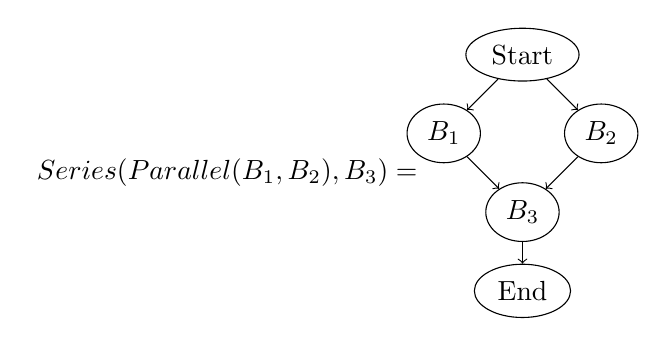
\begin{tikzpicture}
    \node (C) at (-0.75,1.5) { \(Series(Parallel(B_1,B_2), B_3)=\)};
    \node[draw, ellipse] (S)  at (3, 3) {Start};
    \node[draw, ellipse] (B1) at (2, 2) {\( B_1 \)};
    \node[draw, ellipse] (B2) at (4, 2) {\( B_2 \)};
    \node[draw, ellipse] (B3) at (3, 1) {\( B_3 \)};
    \node[draw, ellipse] (T)  at (3, 0) {End};

    \draw[->] (S) to (B1);
    \draw[->] (S) to (B2);
    \draw[->] (B1) to (B3);
    \draw[->] (B2) to (B3);
    \draw[->] (B3) to (T);

\end{tikzpicture}

\end{document}



